%% ma: L10-B02-0013
%% lop: 10
%% chuong: 1
%% bai: 2
%% dang: 10.2.8
%% loai: TN4
%% muc: TH
%% dap_an: "D"
%% nguon: "Ảnh giáo viên gửi 10/10/2026 (ThS. Nguyễn Hoàng Việt, Chương 2 Tập hợp), A-Đề 1, Phần 1 Câu 11"
%% kien_thuc: "Bài 2 (tập hợp và các phép toán trên tập hợp)"
%% trang_thai: cho-duyet
%% ly_do: "Dạng toán mới đề xuất 10.2.8: biểu đồ Ven"
%% ghi_chu: "Hình dựng lại từ biểu đồ gốc; nhãn tập lớn nhất trong ảnh gốc đọc là X (ảnh mờ, in giống chữ C) theo cách dùng C_X A trong các phương án; A và B nằm rời nhau trong X"
\begin{ex}
Cho các tập hợp $A$, $B$, $X$ được biểu diễn trong biểu đồ Ven như sau. Khẳng định nào sau đây \textbf{sai}?
\begin{center}
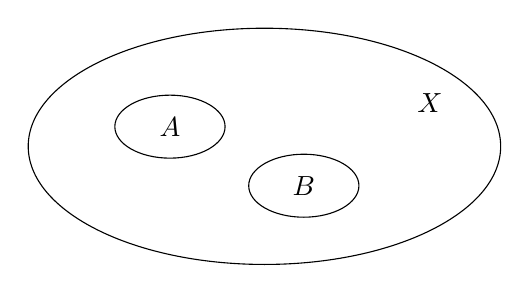
\begin{tikzpicture}
  \draw (0,0) ellipse (3 and 1.5);
  \node at (2.1,.55) {$X$};
  \draw (-1.2,.25) ellipse (.7 and .4); \node at (-1.2,.25) {$A$};
  \draw (.5,-.5) ellipse (.7 and .4); \node at (.5,-.5) {$B$};
\end{tikzpicture}
\end{center}
\choice{$B\subset C_XA$}{$A\cap B=\varnothing$}{$A\subset C_XB$}{\True $A\cup B=X$}
\loigiai{Từ biểu đồ: $A$, $B$ nằm trong $X$ và không có phần chung. Do đó $A\cap B=\varnothing$, $B\subset C_XA$, $A\subset C_XB$ đều đúng. $A\cup B=X$ sai vì $X$ còn có phần tử không thuộc $A$ và không thuộc $B$.}
\end{ex}
